\section{Hardware Results by Regime}
\label{sec:results}
% Evidence: M4-24, M4-HE, RTX-cpu_k2, RTX-rtx_k2, B570-SERIAL, 358H-CPU/NPU.
\begin{table*}[t]
\caption{Headline decode outcomes. Speedup is baseline/speculative time, aggregated by the campaign's frozen prompt estimator. Brackets are 95\% prompt-bootstrap CIs. Exact pairs and faster prompts are separate metrics. B570 timing is diagnostic, despite a reported CI.}
\label{tab:headlines}
\centering
\begin{tabular}{>{\raggedright\arraybackslash}p{2.0in}>{\raggedright\arraybackslash}p{1.70in}>{\raggedright\arraybackslash}p{0.64in}>{\raggedright\arraybackslash}p{0.72in}>{\raggedright\arraybackslash}p{0.64in}}
\toprule
Path / workload & Speedup [95\% CI] & Exact pairs & Faster prompts & Class \\
\midrule
M4 representative 24Q & \MRepSpeed\ [\MRepLo, \MRepHi] & \MRepExact/\MRepPairs & \MRepFaster/\MRepN & Primary \\
M4 HumanEval fixed-$k=2$ & \MHEspeed\ [\MHElo, \MHEhi] & \MHEexact/\MHEpairs & \MHEfaster/\MHEprompts & Primary \\
CPU to RTX 5070 Ti Laptop & \RTXcpuSpeed\ [\RTXcpuLo, \RTXcpuHi] & 90/90 & 0/30 & Second. \\
RTX 5070 Ti Laptop to itself & \RTXgpuSpeed\ [\RTXgpuLo, \RTXgpuHi] & 90/90 & 0/30 & Second. \\
B570 serialized fallback & \BSpeed\ [\BLo, \BHi] & \BExact/90 & 0/30 & Diag. \\
358H CPU draft & \HcpuSpeed\ [\HcpuLo, \HcpuHi] & 90/90 & 0/30 & Primary \\
358H NPU draft & \HnpuSpeed\ [\HnpuLo, \HnpuHi] & 90/90 & 0/30 & Primary \\
\bottomrule
\end{tabular}
\end{table*}

\subsection{M4: workload-conditioned profitability}
% Immutable scientific style asset from PR #19; v0.3 caption preserves transferred qualifications.
\begin{figure}[t]
\centering
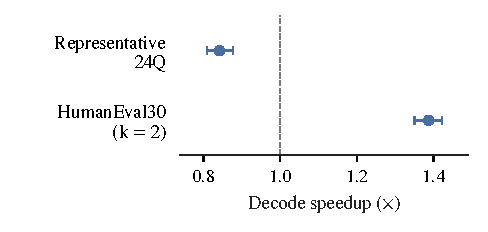
\includegraphics[width=\columnwidth]{../figures/style_v04/pdf/m4.pdf}
\caption{\textbf{Opposite profitability regimes on the same tested M4 stack}. Representative 24Q yields 0.842$\times$ [0.809, 0.877], while the separately preregistered HumanEval30 fixed-$k=2$ study yields 1.387$\times$ [1.351, 1.422]. Points are campaign prompt geometric means of paired decode speedups; intervals are campaign-specific 95\% prompt-bootstrap intervals. The dashed line marks parity. Both paths satisfy token equality (72/72 and 90/90 pairs), which is not functional HumanEval pass@$k$. These are separate studies, not a paired between-workload comparison; differing workloads and session conditions do not isolate workload-only causality.}
\label{fig:m4}
\end{figure}

The representative frozen M4 sample produces \MRepSpeed$\times$ speedup (95\% CI [\MRepLo, \MRepHi]), with \MRepExact/\MRepPairs\ exact pairs and only \MRepFaster/\MRepN\ prompts faster. The separately preregistered HumanEval fixed-$k=2$ study produces \MHEspeed$\times$ [\MHElo, \MHEhi], with \MHEexact/\MHEpairs\ exact pairs and \MHEfaster/\MHEprompts\ prompts faster. Figure~\ref{fig:m4} retains both; the positive code-conditioned result does not replace or pool with the negative representative result.

This establishes existence of an exact profitable workload regime on the measured M4 stack. It does not establish general M4 profitability or isolate unified memory as its cause. The workloads and session conditions differ, and the earlier discovery effect size is not promoted as a confirmatory estimate. Historical MLX failures also do not negate the final qualified Q8\_0 Metal result.

For primary fixed-$k=2$ HumanEval, the package-efficiency ratio (baseline/speculative J per output token) is \MHEenergy$\times$ [\MHEenergyLo, \MHEenergyHi]. The interval includes one: energy is neutral within uncertainty. The registered $p_{\min}=0.9$ condition has secondary energy evidence, discussed separately in the appendix. The preregistered corrected synthetic ceiling was not executed. We retain that deviation rather than treating the earlier synthetic diagnostic as its replacement.

\subsection{RTX 5070 Ti Laptop: exact controls remain negative}
The serialized CPU-to-RTX control reaches \RTXcpuSpeed$\times$ [\RTXcpuLo, \RTXcpuHi], while the same-GPU draft control reaches \RTXgpuSpeed$\times$ [\RTXgpuLo, \RTXgpuHi]. Both are \RTXexact/90\ exact and accelerate zero of 30 prompts. The higher speed of same-GPU placement shows that placement and associated integration costs matter, but its continued loss rules out transfer as the sole explanation.

These controls are deliberately secondary. They qualify a slower path after the native fast attempt failed; they are not a rescued primary success. The verification microbenchmark explains lost batching opportunity, while the complete end-to-end controls include drafting and integration. We cannot recover a full $\rtarget$ decomposition by substituting the forward-only ratio into Equation~\ref{eq:normalized}.

\subsection{Arc B570: correctness-blocked diagnostics}
Neither the fast path nor the serialized fallback supports a workload-global admissible optimization result. The latter's diagnostic speedup is \BSpeed$\times$ [\BLo, \BHi], with zero of 30 prompts faster. That interval describes timing on a partially mismatching path; its precision does not turn it into an admissible speed claim. The formal failure and stop rule remain the platform result. Board-energy observations likewise remain diagnostic and boundary-limited.

This negative control matters because it prevents an attractive simplification: selecting serialized verification is not by itself a sufficient correctness policy. Qualification must cover the actual path and intended workload. Exact subsets may be descriptively useful, but conditioning on those subsets after the run cannot establish global performance.

\subsection{Core Ultra X7 358H: realized state changes the cost}
% Evidence: 358H-ISOLATED and 358H-CPU/NPU; boundaries deliberately separate.
\begin{figure*}[t]
\centering
\begin{tikzpicture}
\begin{axis}[name=left,width=3.05in,height=2.25in,xmode=log,log basis x=2,xtick={512,2048,8192},xticklabels={512,2048,8192},xlabel={Isolated draft context (tokens)},ylabel={Steady-state draft tokens/s},ymin=0,ymax=115,legend style={at={(.5,1.02)},anchor=south,legend columns=2},grid=major]
\addplot+[blue!70!black,mark=*] table[x=context,y=CPU] {figures/04_isolated.dat};\addlegendentry{CPU}
\addplot+[orange!80!black,mark=square*] table[x=context,y=NPU] {figures/04_isolated.dat};\addlegendentry{NPU}
\end{axis}
\begin{axis}[at={(left.east)},anchor=west,xshift=.70in,width=3.05in,height=2.25in,ybar stacked,bar width=22pt,symbolic x coords={CPU,NPU},xtick=data,xlabel={Realized Phase-3 draft path},ylabel={Seconds / request},ymin=0,ymax=32,legend style={at={(.5,1.02)},anchor=south,legend columns=1},ymajorgrids]
\addplot+[fill=orange!65,draw=black] table[x=device,y=draft] {figures/04_realized.dat};\addlegendentry{Replay + proposal}
\addplot+[fill=blue!45,draw=black] table[x=device,y=target] {figures/04_realized.dat};\addlegendentry{Complete target side}
\addplot+[fill=black,draw=black] table[x=device,y=residual] {figures/04_realized.dat};\addlegendentry{Residual}
\end{axis}
\end{tikzpicture}
\caption{Why does isolated NPU speed not survive integration on 358H? Left: median isolated steady-state draft throughput (five repetitions/cell), excluding the first-token cost. Right: arithmetic mean complete post-prefill request time over 90 observations/path. CPU time is target-side dominated (\HcpuTarget\%); NPU time is replay-plus-proposal dominated (\HnpuDraft\%). Residuals are only \HcpuResidual\%/\HnpuResidual\% and visually negligible. Separate boundaries preclude interpreting left-panel throughput as realized draft cost.}
\label{fig:state}
\end{figure*}

The closed Phase-3 heterogeneous runner is exact on both CPU and NPU drafting: \HExact/90\ pairs per path, with zero of 30 prompts faster. CPU achieves \HcpuSpeed$\times$ [\HcpuLo, \HcpuHi]; NPU achieves \HnpuSpeed$\times$ [\HnpuLo, \HnpuHi]. The direct round records show mean committed progress $C=\HcpuC$ and $\HnpuC$, respectively, approximately 2.46. This is complete committed output, not the accepted-draft counter used in older native records.

The target maintains persistent state, evaluates proposals, removes invalid candidate state when needed, and decodes correction or bonus output. Its complete measured region accounts for \HcpuTarget\% of CPU-path speculative time. The NPU path instead spends \HnpuDraft\% in the synchronous OpenVINO call that replays the full committed prefix and generates a proposal. Replay and proposal are inseparable within this measurement; we do not invent a replay-only value. Residual orchestration occupies only \HcpuResidual\% and \HnpuResidual\%, so it cannot explain the main loss.

Figure~\ref{fig:state} separates isolated steady-state throughput from this realized request decomposition. The isolated NPU draft can outperform the CPU at the tested contexts, but this advantage does not survive the qualified state interface. The conclusion concerns that implementation, not insufficient NPU compute capability. A state-persistent intervention has not been implemented or measured.

Using arithmetic totals at a common boundary reconstructs Equation~\ref{eq:normalized}. CPU has $(\dreal,\rtarget,X)=(\HcpuD,\HcpuR,\HcpuX)$ and aggregate speedup \HcpuAggregate$\times$; NPU has $(\HnpuD,\HnpuR,\HnpuX)$ and \HnpuAggregate$\times$. These agree with the ratios of total baseline/speculative times. They intentionally differ from the primary prompt-level geometric means in Table~\ref{tab:headlines}.

The earlier Phase-2 screen combined isolated drafting and a target-forward proxy under favorable residual-cost assumptions. It was an eligibility screen, not a validated end-to-end prediction. Phase 3 shows why those proxies must be replaced with complete target-side work and realized stateful draft cost. No end-to-end Phase-3 energy result is claimed, and source reconstruction retains its \texttt{STRONGLY\_SUPPORTED} qualification.

\subsection{Stable hardware-study conclusion}
\label{sec:hardwareconclusion}
% Selected immutable publication asset from PR #17; caption adapted from the integration kit.
\begin{figure*}[t]
\centering
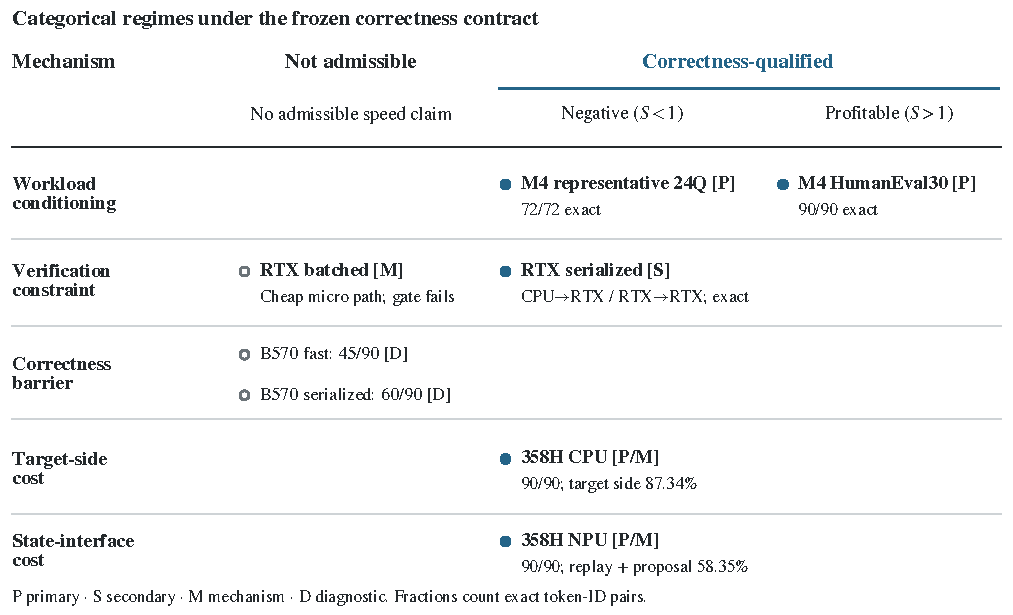
\includegraphics[width=\textwidth]{../figures/pdf/figure5.pdf}
\caption{\textbf{Evidence inventory across tested regimes}. Categorical columns distinguish globally blocked paths from exact negative and profitable regimes. Rows annotate observed constraints rather than define an exhaustive taxonomy. Both B570 paths remain diagnostic and globally inadmissible. RTX serialized controls are secondary evidence; 358H outcome and decomposition support primary and mechanism claims, respectively. Empty cells indicate no displayed case, not impossibility. No hardware ordering or continuous correctness metric is implied.}
\label{fig:regimes}
\end{figure*}

The tested systems expose four useful regimes: profitable and exact, exact but unprofitable, physically cheap but correctness-inadmissible, and state-interface-bound. Figure~\ref{fig:regimes} maps them categorically; regimes can overlap and are not hardware ranks. Correctness determines which measured paths can support an optimization claim, then realized costs determine whether their committed progress pays. This conclusion requires neither a successful future prototype nor extrapolation from one workload to an entire device family.
